\documentclass[12pt,french]{article}
\input preambule_2013

\newcounter{exoc}
\newenvironment{exoc}[1]{%
  \refstepcounter{exoc}\textbf{Exercice \theexoc} :\hfill {\textbf{(#1)}}\par
  \medskip}%
{\medskip}

\setlength{\textheight}{27cm}% Hauteur de la zone de texte

\begin{document}


\pieddepage{}{}{}

\begin{center}
\begin{tabularx}{\textwidth}{|>\centering m{2.5cm}|>\centering X|>{\centering\arraybackslash} m{2.5cm}|}
	\hline
		1\iere \bsc{S.t.i.2d.} &  Lundi 24 mars \np{2014} & \textbf{Second degré} \\
	\hline
		\multicolumn{3}{|c|}{\bsc{Contrôle de mathématiques}} \\
	\hline
        \multicolumn{1}{|r}{\bsc{Nom}:} & \multicolumn{2}{l|}{} \\
		\multicolumn{1}{|r}{Prénom:} & \multicolumn{2}{l|}{} \\
	\hline
        \multicolumn{3}{|l|}{\bfseries Note et observations :} \\[1cm]
    \hline
\end{tabularx}\bigskip

{\itshape
La qualité et la précision de la rédaction seront prises en compte dans l'appréciation des copies.\par
Le barème est indicatif.
}
\end{center}

\begin{exoc}{3 + 1 + 0,5 + 1,5 = 6 points}
    On utilise un tableur pour déterminer les racines de polynômes écrits sous la forme $ax^2 + bx+c$.
    \[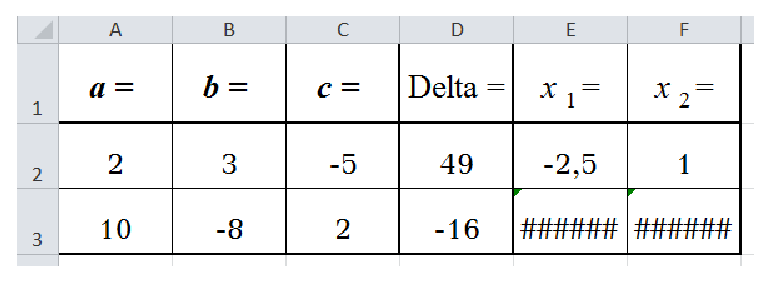
\includegraphics[scale=0.7]{Second_Degre_Excel.eps}\]
    \begin{enumerate}
        \item En détaillant les calculs, retrouver les résultats affichés dans les cellules \verb!D2!, \verb!E2! et \verb!F2!.
        \item En rappelant les formules du cours, donner alors la factorisation du polynôme \[A(x) = 2x^2 + 3x - 5.\]
        \item Comment interpréter les symboles \verb!######! obtenus dans les cellules \verb!E3! et \verb!F3! ?
        \item On appelle $B$ le polynôme défini par les c{\oe}fficients de la ligne \verb!3!.
            \begin{enumerate}
                \item Donner l'expression du polynôme $B$ en fonction de $x$.
                \item Sans aucun calcul ni tableau de signes, en utilisant uniquement le tableur, déterminer le signe de $B$ en fonction de $x$.\par \textbf{Attention.} Une réponse non justifiée ne rapportera aucun point, même si elle est juste !
            \end{enumerate}
    \end{enumerate}
\end{exoc}\[*\]

\begin{exoc}{2 + 2 + 2 = 6 points}
    On considère la fonction polynôme $f$ telle que :
    \[\left\{\begin{array}{l}
            f(x) = ax^2 + bx + c \quad \text{pour tout } x \in \R\ ; \\
            f(0) = -1\ ;\\
            f(1) = 1,5 \quad \text{et} \\
            f(4) = 21.
    \end{array}\right.\]

    \begin{enumerate}
        \item Démontrer que $f(x) = x^2 + 1,5x - 1$.
        \item Résoudre l'équation $f(x) = 0$.
        \item Dresser le tableau de signes de $f$ sur $\R$ et résoudre $f(x) \geqslant 0$.
    \end{enumerate}
\end{exoc}

\vfill

\begin{center}
    \bfseries
    Tourner la page !
\end{center}

\clearpage

\begin{exoc}{1 + 0,5 + 2 + 2,5 + 2 = 8}
Dans le cadre d'un atelier expérimental, un groupe de lycéens a fabriqué des micro-fusées.\par
Lors d'un essai, ils ont lancé verticalement une de ces micro-fusées à la vitesse de $20~m\cdot s^{-1}$.\par
La hauteur $h$ (en mètres) atteinte par la micro-fusée en fonction du temps $t$ (en secondes) est donnée par : \[h(t) = -5t^2 + 20t + 1,6.\]\bigskip

\begin{center}
    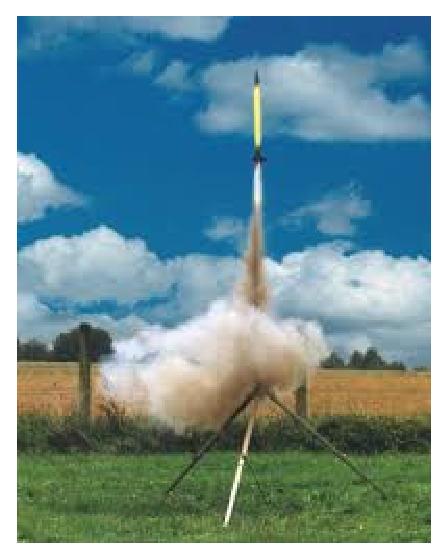
\includegraphics[height=7cm]{fusee.eps}\qquad\qquad
    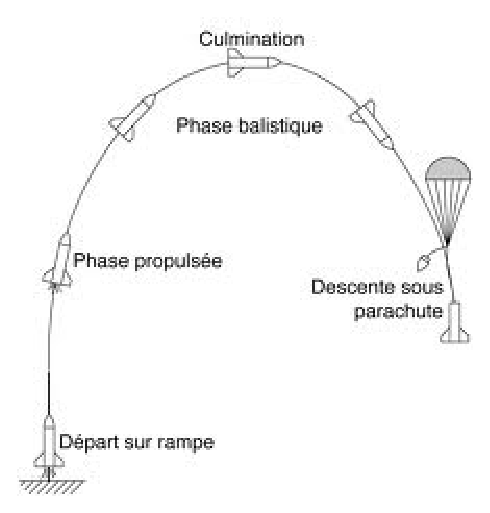
\includegraphics[height=7cm]{fusee_parabole.eps}
\end{center}\bigskip

\begin{enumerate}
    \item Déterminer par le calcul la hauteur de la micro-fusée au bout d'une seconde puis au bout de trois secondes.
    \item Quelle est la hauteur de la fusée au moment du lancement ? Justifier la réponse.
    \item Déterminer par le calcul la hauteur maximale $H_{max}$ atteinte par la micro-fusée.
    \item Déterminer par le calcul les deux solutions $h_1$ et $h_2$ de l'équation $h(t) = 0$.\par
        Les résultats seront arrondis au dixième près.
    \item Les solutions ont-elles une signification réelle dans ce contexte là ?\par
        Si oui, donner l'interprétation de la solution. Si non, expliquer pourquoi.
\end{enumerate}

\end{exoc}

\end{document} 